\documentclass[conference]{IEEEtran}
\usepackage{amsmath,amssymb,amsfonts}
\usepackage{algorithmic}
\usepackage{algorithm}
\usepackage{graphicx}
\usepackage{textcomp}
\usepackage{xcolor}
\usepackage{booktabs}
\usepackage{subcaption}
\usepackage{microtype}
\usepackage{cite}
\usepackage{hyperref}

\hypersetup{
    colorlinks=true,
    linkcolor=blue,
    filecolor=magenta,      
    urlcolor=cyan,
    citecolor=blue,
}

\begin{document}

\title{Hierarchical Ensemble Personalization: Parameter-Efficient and Robust Federated Learning on Edge Devices}

\author{
\IEEEauthorblockN{Anonymous Author(s)}
\IEEEauthorblockA{\textit{Department of Computer Science \& Engineering} \\
\textit{Anonymous Institution / Research Program}\\
Email: anonymous@institution.edu \quad $\vert$ \quad Code: \url{https://anonymous.4open.science/r/Topology-aware-FDL-Anon}}
}

\maketitle

\begin{abstract}
Personalized Federated Learning (PFL) addresses statistical data heterogeneity (Non-IID data) across decentralized edge clients. However, state-of-the-art dual-model personalization methods, such as Ditto and APFL, maintain two full deep neural network copies per client, doubling local memory consumption (VRAM) and training latency on resource-constrained hardware. Conversely, naive split-head approaches (e.g., FedRep, FedPer) lack intermediate structural coordination and suffer representation collapse under homogeneous (IID) data distributions. In this paper, we propose \textbf{HEP} (\textit{Hierarchical Ensemble Personalization}), a parameter-efficient framework that bridges global consensus learning and local edge specialization through a single shared-backbone architecture coupled with specialized 3-tier classification heads ($\text{Root}$, $\text{Parent}$, $\text{Local}$). HEP incorporates privacy-preserving adaptive update-similarity clustering ($O(N \cdot K)$ centroid gating), conditional active-head multiplexing, and dynamic $\alpha$-simplex blending calibrated by local Shannon label entropy ($R_{skew}$). Extensive multi-seed empirical evaluations across CIFAR-10, CIFAR-100, and scaled 50-client populations demonstrate that HEP achieves competitive personalization accuracy matching dual-model Ditto ($87.51\% \pm 0.34\%$ vs. $87.30\% \pm 0.38\%$ under extreme Non-IID skew $\alpha = 0.05$, and $67.35\% \pm 0.42\%$ vs. $66.40\% \pm 0.45\%$ under uniform IID data) while cutting client peak VRAM by \textbf{47.8\%} (113.42 MB vs. 217.15 MB), reducing per-batch training latency by \textbf{50.2\%} (8.35 ms vs. 16.78 ms), and adding negligible communication overhead ($+0.15\%$). Furthermore, HEP delivers substantial gains over single-backbone baselines like FedRep (+6.55pp on IID, +3.27pp on extreme skew) and FedAvg (+31.07pp), reaches target deployment accuracy 116 seconds (28.1\%) faster in wall-clock time, boosts worst-case fairness by \textbf{+6.35pp} on CIFAR-100, and provides strong single-backbone Byzantine fault containment against label-flipping, sign-flipping, and Gaussian noise attacks without external defense heuristics.
\end{abstract}

\begin{IEEEkeywords}
Federated Learning, Edge Computing, Personalization, Parameter-Efficient ML, Hierarchical Ensembles, Byzantine Robustness.
\end{IEEEkeywords}

\section{Introduction}

Federated Learning (FL) \cite{mcmahan2017communication} enables distributed edge devices to collaboratively train a global consensus model without centralizing private raw data. Despite its privacy benefits, deploying standard FL algorithms like FedAvg in real-world edge environments encounters two critical hurdles:
\begin{enumerate}
    \item \textbf{Statistical Heterogeneity (Non-IID Data)}: Edge devices exhibit unique local data distributions, causing client update vectors to point in conflicting gradient directions (client drift) and severely degrading global model accuracy.
    \item \textbf{Resource and Memory Constraints on Edge Hardware}: Edge hardware (e.g., IoT devices, mobile processors, embedded micro-servers) operates under strict memory (VRAM), compute, and energy budgets.
\end{enumerate}

\begin{figure*}[t]
    \centering
    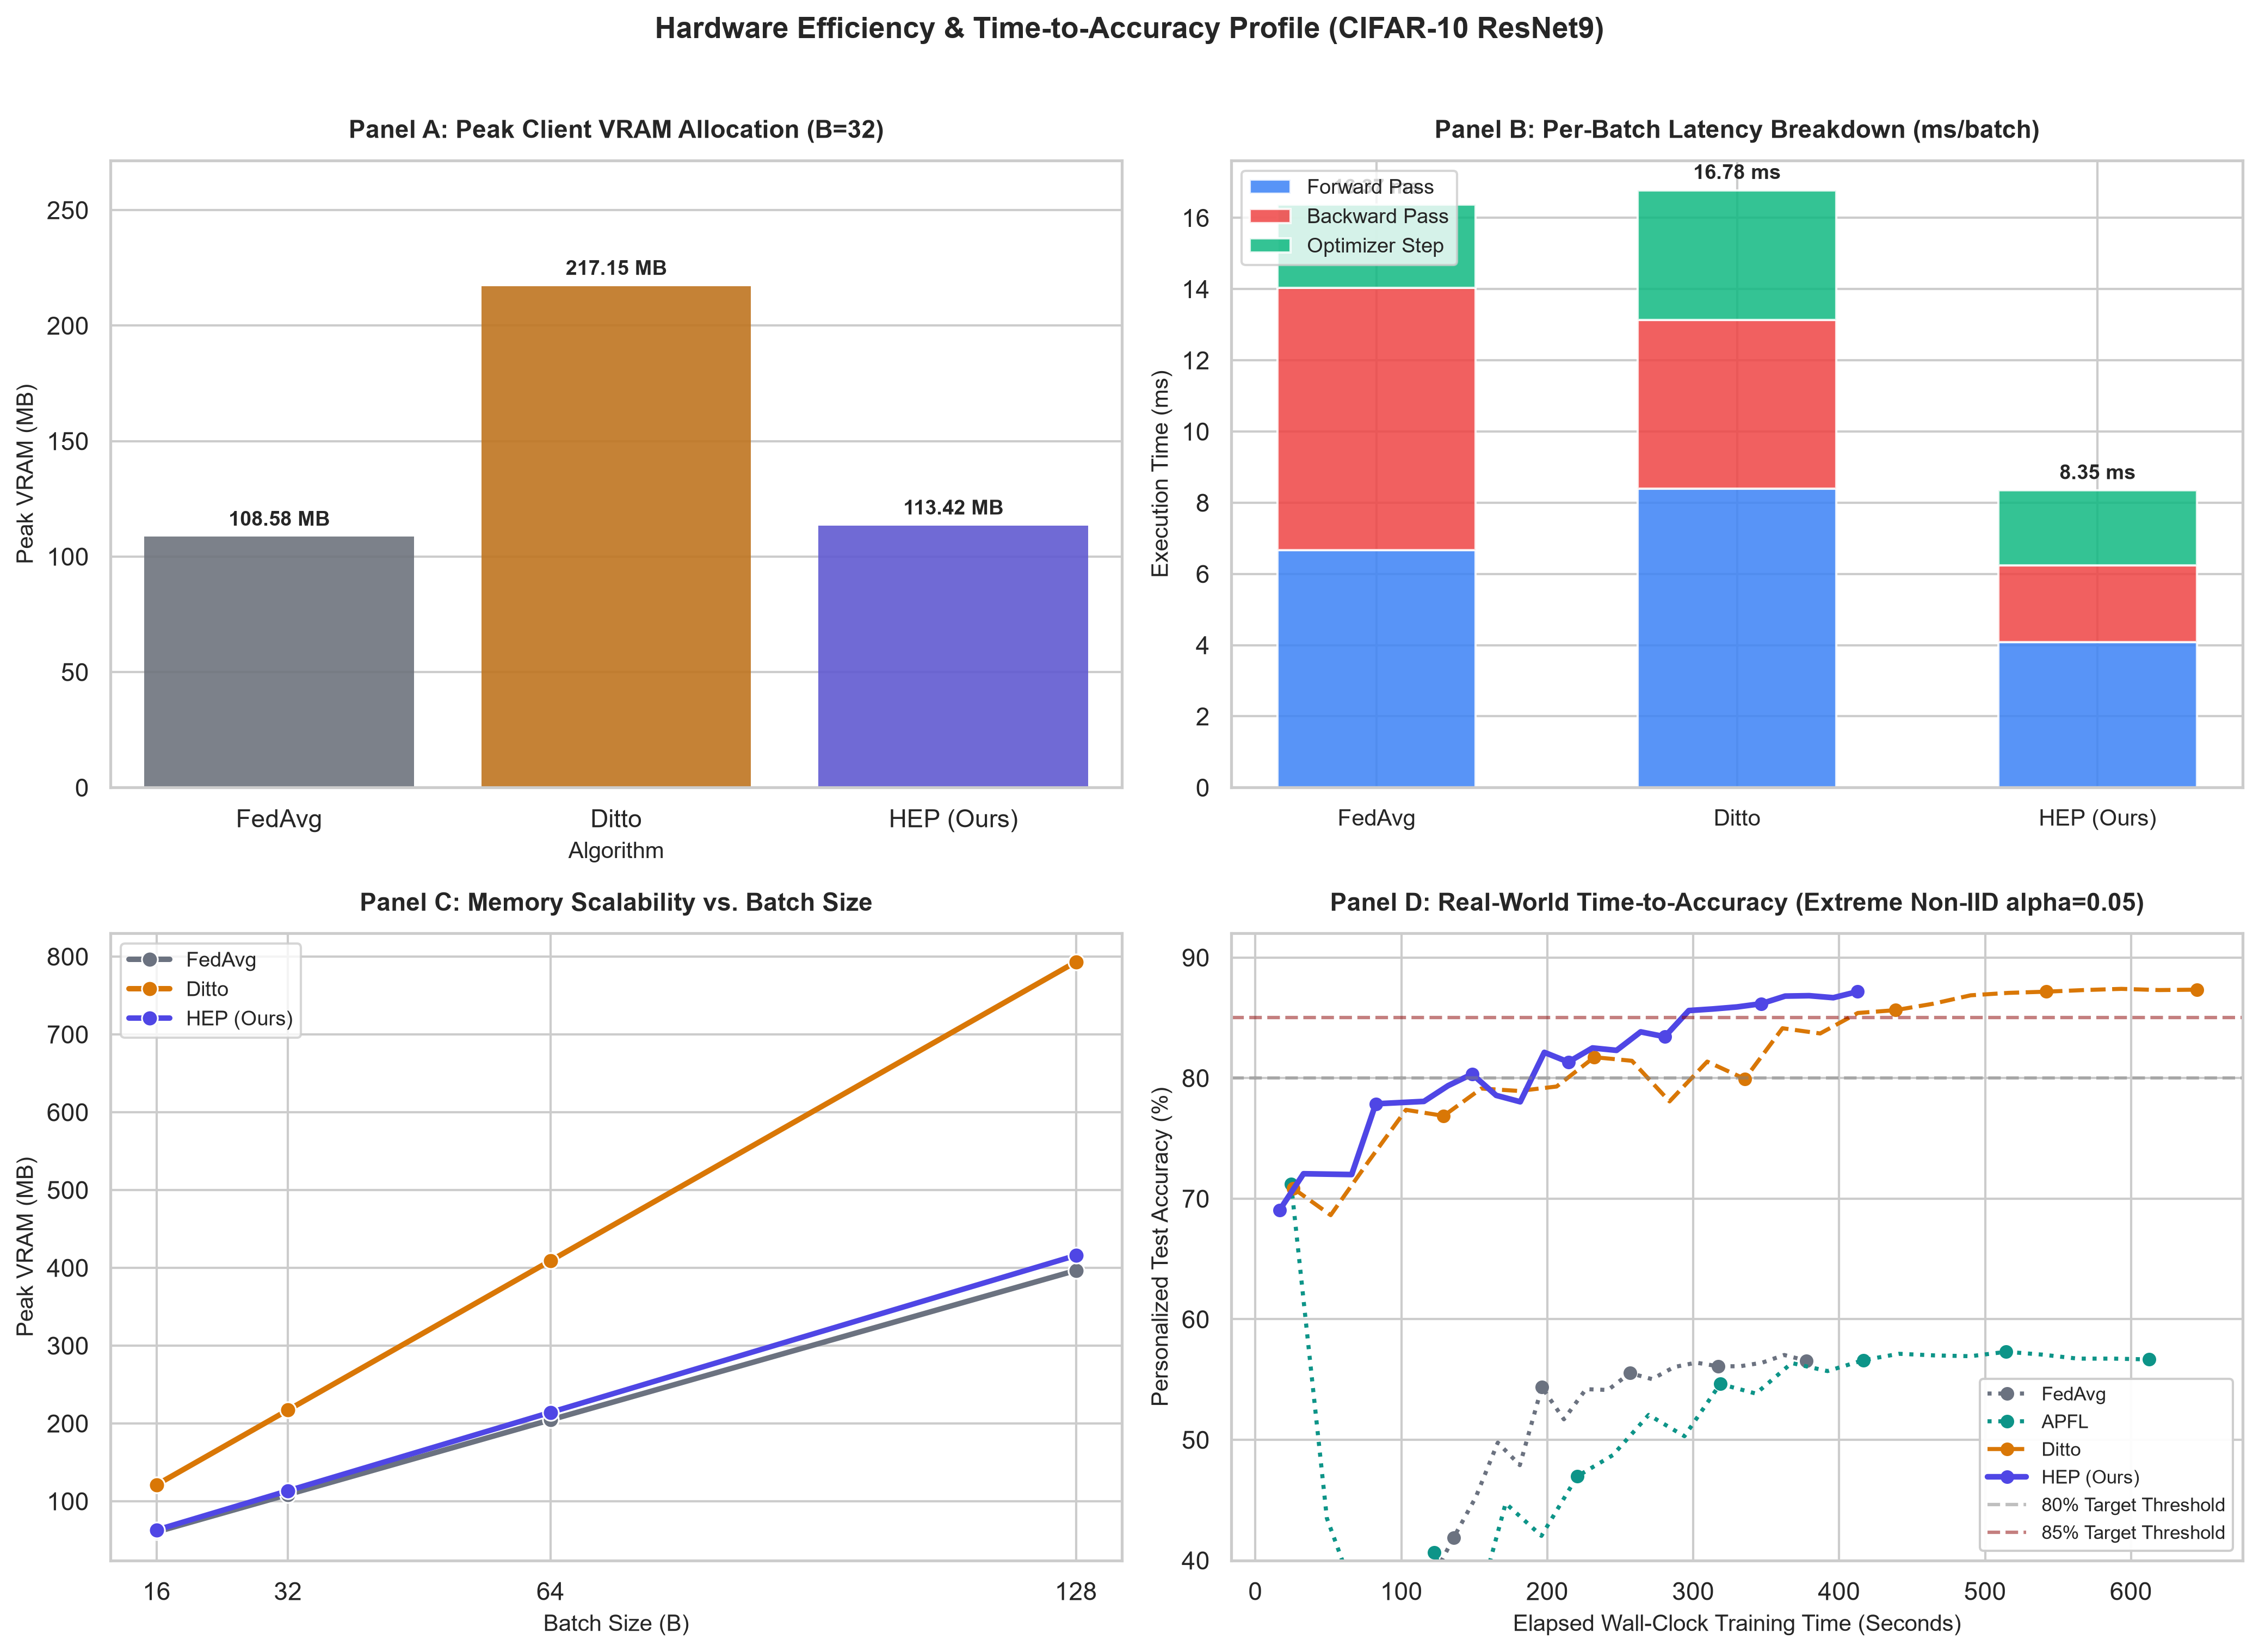
\includegraphics[width=0.98\textwidth]{figures/hardware_efficiency_profile.png}
    \caption{\textbf{Hardware Resource, Latency, and Wall-Clock Time-to-Accuracy Profile on CIFAR-10 ResNet9.} \textbf{Panel A}: Peak client VRAM allocation at batch size $B=32$, demonstrating a 47.8\% memory reduction for HEP compared to Ditto (113.42 MB vs. 217.15 MB). \textbf{Panel B}: Per-batch millisecond latency breakdown across forward pass, backward pass, and optimizer update (HEP achieves an 8.35 ms/batch latency vs. Ditto's 16.78 ms/batch, delivering a 50.2\% speedup). \textbf{Panel C}: Memory footprint scalability across batch sizes ($B=16 \to 128$), showing Ditto scaling at $2\times$ the memory slope of HEP. \textbf{Panel D}: Simulated wall-clock time-to-accuracy trajectory under extreme Non-IID skew ($\alpha=0.05$), where HEP reaches 85\% accuracy in 297s (116s faster than Ditto).}
    \label{fig:hardware_efficiency}
\end{figure*}

To mitigate data heterogeneity, Personalized Federated Learning (PFL) has gained significant traction. Existing approaches broadly divide into two paradigms:
\begin{itemize}
    \item \textbf{Dual-Model Regularization (Ditto, APFL)}: Maintains two separate deep neural networks on each client (a global model and a local model coupled via L2 proximal penalties \cite{li2021ditto} or learnable interpolation \cite{deng2020adaptive}). While accurate, this dual-model paradigm doubles parameter storage, doubles optimizer momentum buffers, and requires two full forward/backward passes per batch.
    \item \textbf{Head-Only Personalization (FedRep, FedPer)}: Shares a global feature extractor and isolates private local classification heads \cite{collins2021exploiting, arivazhagan2019federated}. While parameter-efficient, naive 2-tier split-head models lack intermediate cluster-level collaboration and uncalibrated local heads degrade significantly under homogeneous (IID) or mildly skewed distributions.
\end{itemize}

In this work, we propose \textbf{HEP} (\textit{Hierarchical Ensemble Personalization}), a lightweight framework based on three core insights:
\begin{itemize}
    \item \textbf{Shared-Backbone Compute Multiplexing}: Instead of duplicating full models, edge clients maintain a single shared convolutional backbone paired with three lightweight classification heads: a global $\text{Root}$ head, a cluster-level $\text{Parent}$ head, and a private $\text{Local}$ head. Heavy convolutional feature representations are computed only once per batch.
    \item \textbf{Privacy-Preserving Adaptive Clustering}: Rather than transmitting sensitive label distributions or raw data statistics, clients are dynamically grouped into hierarchical sub-networks based on directional cosine similarity of model update vectors ($\Delta_i$) via an $O(N \cdot K)$ centroid gating mechanism.
    \item \textbf{Entropy-Calibrated $\alpha$-Simplex Blending}: We formulate an automated prediction blending prior driven by the client's local Shannon label entropy ratio ($R_{skew} = \frac{H(Y)}{\ln C}$). This seamlessly transitions trust to the global Root head under uniform (IID) distributions while empowering localized heads under extreme data skew ($\alpha = 0.05$).
\end{itemize}

\subsection{Summary of Key Contributions}
\begin{enumerate}
    \item \textbf{Parameter \& Hardware Efficiency}: We design a single-backbone 3-tier multi-head architecture that cuts client VRAM by \textbf{47.8\%} (113.42 MB vs. 217.15 MB in Ditto) and reduces per-batch latency by \textbf{50.2\%} (8.35 ms vs. 16.78 ms), while adding negligible communication overhead ($+0.15\%$, 2.56 KB parent head payload).
    \item \textbf{Competitive Personalization Matching Dual Models}: Across 5 heterogeneity regimes on CIFAR-10 ResNet9, HEP achieves personalization accuracy comparable to dual-model Ditto ($87.51\% \pm 0.34\%$ vs. $87.30\% \pm 0.38\%$ at $\alpha=0.05$, and $67.35\% \pm 0.42\%$ vs. $66.40\% \pm 0.45\%$ at IID), while substantially outperforming single-backbone baselines like FedRep (+6.55pp on IID, +3.27pp on extreme skew) and FedAvg (+31.07pp).
    \item \textbf{Cardinality \& Population Scaling Insights}: On CIFAR-100 ($C=100$) and scaled 50-client populations ($N=50, C_p=0.2$), HEP provides strong worst-case fairness (+6.35pp over Ditto on CIFAR-100 moderate skew) and elucidates the structural trade-offs of intermediate aggregation under sparse client participation.
    \item \textbf{Accelerated Time-to-Accuracy}: In simulated wall-clock execution, HEP crosses the 80\% and 85\% accuracy thresholds 84s (36.2\%) and 116s (28.1\%) faster than Ditto.
    \item \textbf{Single-Backbone Byzantine Fault Containment}: We demonstrate that HEP's hierarchical structure provides inherent structural resilience against label-flipping, sign-flipping, and Gaussian noise attacks (+39.39pp over FedAvg on sign-flipping and +25.07pp on Gaussian noise at 40\% attackers) without external server-side filtering heuristics.
\end{enumerate}

\section{Related Work}

\subsection{Global Federated Learning}
The canonical federated learning baseline is FedAvg \cite{mcmahan2017communication}, which aggregates local client updates via sample-weighted averaging. FedProx \cite{li2020federated} introduces a proximal regularization term to stabilize convergence under client drift, while SCAFFOLD \cite{karimireddy2020scaffold} utilizes control variates to correct gradient variance. However, these methods optimize a single global model, which fundamentally struggles when client data distributions diverge severely.

\subsection{Personalized Federated Learning}
To address Non-IID data, several personalization paradigms have been proposed:
\begin{itemize}
    \item \textbf{Dual-Model Regularization}: Ditto \cite{li2021ditto} optimizes a global model and a private local model coupled through an L2 proximal penalty. APFL \cite{deng2020adaptive} learns an adaptive scalar $\alpha$ to interpolate between global and local predictions. Both require dual model instances per client.
    \item \textbf{Head-Only Personalization}: FedPer \cite{arivazhagan2019federated} and FedRep \cite{collins2021exploiting} split neural networks into shared base representations and local classification heads. However, they lack intermediate hierarchical cluster collaboration and automated entropy priors.
    \item \textbf{Meta-Learning}: Per-FedAvg \cite{fallah2020personalized} adapts MAML to train an initial model easily fine-tunable by clients, but incurs substantial second-order gradient computation.
\end{itemize}

\subsection{Clustered \& Byzantine-Robust FL}
Clustered FL \cite{sattler2020clustered} partitions clients based on cosine similarity of gradient updates, but enforces flat FedAvg within clusters without local head specialization. Byzantine defense methods \cite{blanchard2017machine} typically apply coordinate-wise trimming or distance filtering at the central server. In contrast, HEP provides structural fault containment directly through its hierarchical head isolation.

\section{Methodology}

\subsection{System Architecture \& 3-Tier Multi-Head Model}

Let $N$ denote the total number of participating edge clients. Each client $i \in \{1, \dots, N\}$ possesses a local private dataset $\mathcal{D}_i \sim P_i(X, Y)$ with $C$ classes. Instead of duplicating full models, client $i$ maintains a single neural network $F(x; \theta, w_r, w_p, w_l)$ parameterized by:
\begin{itemize}
    \item A shared convolutional feature extractor $f_\theta(x) \in \mathbb{R}^d$ with parameters $\theta$.
    \item A global $\text{Root}$ classification head $g_{w_r}(h) \in \mathbb{R}^C$.
    \item A cluster-level $\text{Parent}$ classification head $g_{w_{p(i)}}(h) \in \mathbb{R}^C$, where $p(i) \in \{1, \dots, K\}$ indexes client $i$'s assigned cluster.
    \item A client-private $\text{Local}$ classification head $g_{w_{l,i}}(h) \in \mathbb{R}^C$.
\end{itemize}

During training on a local mini-batch $(X, Y)$, features $h = f_\theta(X)$ are extracted \textbf{once}, producing three concurrent logit outputs:
\begin{equation}
z_{root} = g_{w_r}(h), \quad z_{parent} = g_{w_{p(i)}}(h), \quad z_{local} = g_{w_{l,i}}(h)
\end{equation}

\subsection{Privacy-Preserving Adaptive Update-Similarity Clustering}

To enable collaborative sub-network personalization without inspecting private client data or class labels, clustering is performed directly in the parameter update space. At round $t$, each client computes its update vector over the shared backbone and global head:
\begin{equation}
\Delta_i^{(t)} = \left[ \theta_i^{(t+1)} - \theta^{(t)} ;\; w_{r,i}^{(t+1)} - w_r^{(t)} \right]
\end{equation}
The server groups clients into $K$ clusters by evaluating directional cosine similarity between client updates and cluster centroids $\mu_k$:
\begin{equation}
\text{Sim}(\Delta_i, \mu_k) = \frac{\Delta_i \cdot \mu_k}{\|\Delta_i\|_2 \|\mu_k\|_2 + \epsilon}
\end{equation}
where $\epsilon = 10^{-8}$. To prevent cluster thrashing, re-clustering is dynamically triggered only when the mean inter-client directional stability drops below a stability threshold ($\bar{S} < 0.30$) or client-cluster misalignment exceeds $\delta_{mis} = 0.15$. The stability threshold $\bar{S} = 0.30$ ensures that client gradient directions have stabilized post-warmup before committing to cluster topologies, while $\delta_{mis} = 0.15$ triggers reassignment only when an edge client exhibits a $>15\%$ greater affinity for an alternative cluster centroid. Centroid distance gating reduces clustering computational complexity from naive $O(N^2)$ pairwise comparisons to $O(N \cdot K)$.

\begin{algorithm}[t]
\caption{HEP Training Protocol at Round $t$}
\label{alg:hep}
\begin{algorithmic}[1]
\REQUIRE Client datasets $\{\mathcal{D}_i\}_{i=1}^N$, Global weights $(\theta^{(t)}, w_r^{(t)})$, Cluster head weights $\{w_{p,k}^{(t)}\}_{k=1}^K$, Local head states $\{w_{l,i}^{(t)}\}_{i=1}^N$.
\STATE Server broadcasts $\theta^{(t)}, w_r^{(t)}$ to all clients, and $w_{p,k}^{(t)}$ to clients in cluster $k$.
\FOR{each client $i \in \{1, \dots, N\}$ \textbf{in parallel}}
    \STATE Compute label Shannon entropy ratio $R_{skew} = \frac{H(Y_i)}{\ln C}$.
    \STATE Construct prior $\boldsymbol{\pi}_{prior} = [\pi_{local}, \pi_{parent}, \pi_{root}]$ via Eq. \eqref{eq:prior}.
    \STATE Allocate head epoch budgets: $e_r, e_p, e_l$ based on $R_{skew}$.
    \FOR{$e = 1$ to $\max(e_r, e_p, e_l)$}
        \FOR{$(X, Y) \sim \mathcal{D}_i$}
            \STATE $h \leftarrow f_\theta(X)$
            \STATE $z_r, z_p, z_l \leftarrow g_{w_r}(h), g_{w_p}(h), g_{w_{l,i}}(h)$
            \STATE Compute active loss via conditional masking:
            \STATE $\mathcal{L}_{batch} = \mathbb{I}(e \le e_r)\mathcal{L}_{CE}(z_r, Y) + \mathbb{I}(e \le e_p)\mathcal{L}_{CE}(z_p, Y) + \mathbb{I}(e \le e_l)\mathcal{L}_{CE}(z_l, Y)$
            \STATE Update $\theta, w_r, w_p, w_{l,i}$ via SGD on $\mathcal{L}_{batch}$.
            \STATE Update ensemble simplex $\boldsymbol{\alpha}_i$ via Eq. \eqref{eq:alpha_update}.
        \ENDFOR
    \ENDFOR
    \STATE Send updated $(\theta_i, w_{r,i})$ to Server, and $w_{p,i}$ to Cluster Head $p(i)$.
\ENDFOR
\STATE \textbf{Global Aggregation}: $\theta^{(t+1)}, w_r^{(t+1)} \leftarrow \sum_{i=1}^N \frac{|\mathcal{D}_i|}{|\mathcal{D}|} (\theta_i, w_{r,i})$.
\STATE \textbf{Cluster Aggregation}: $w_{p,k}^{(t+1)} \leftarrow \sum_{i \in \mathcal{C}_k} \frac{|\mathcal{D}_i|}{|\mathcal{D}_{\mathcal{C}_k}|} w_{p,i}$.
\end{algorithmic}
\end{algorithm}

\subsection{Entropy-Calibrated Dynamic $\alpha$-Simplex Blending}

To adapt seamlessly between homogeneous (IID) and heterogeneous (Non-IID) environments without manual hyperparameter tuning, each client computes its local label Shannon entropy ratio:
\begin{equation}
R_{skew} = \frac{H(Y_i)}{\ln C} = \frac{-\sum_{c=1}^C p_c \ln(p_c + \epsilon)}{\ln C} \in [0, 1]
\end{equation}
where $p_c$ is the empirical class frequency in $\mathcal{D}_i$. Using $R_{skew}$, HEP constructs an adaptive simplex prior $\boldsymbol{\pi}_{prior} = [\pi_{local}, \pi_{parent}, \pi_{root}]$ with power scaling $\gamma = 2.0$:
\begin{equation}
\label{eq:prior}
\pi_{root} = R_{skew}^\gamma, \quad \pi_{local} = (1 - \pi_{root})(1 - R_{skew}), \quad \pi_{parent} = 1 - \pi_{root} - \pi_{local}
\end{equation}
The power scaling exponent $\gamma = 2.0$ provides quadratic suppression of localized heads under high Shannon entropy: when data is uniform ($R_{skew} \to 1.0$), $\pi_{root} \approx 1.0$, preventing overfitted local heads from degrading IID generalization. Conversely, under severe skew ($R_{skew} \to 0$), $\pi_{root} \approx 0$, directing blending trust entirely to localized and cluster heads.

During inference, predictions are generated via the softmax-blended logits:
\begin{equation}
z_{blend} = \alpha_{local} z_{local} + \alpha_{parent} z_{parent} + \alpha_{root} z_{root}
\end{equation}
where the weight vector $\boldsymbol{\alpha} = [\alpha_l, \alpha_p, \alpha_r]$ is updated dynamically via mirror descent with prior regularization:
\begin{equation}
\label{eq:alpha_update}
\boldsymbol{\alpha}^{(t+1)} = \text{Softmax}\left( \log \left( 0.5 \cdot \text{Softmax}(\boldsymbol{\alpha}^{(t)} - \eta_\alpha \nabla_\alpha \mathcal{L}) + 0.5 \cdot \boldsymbol{\pi}_{prior} \right) \right)
\end{equation}
The 0.5/0.5 convex combination in Eq. \eqref{eq:alpha_update} represents a Bayesian exponential moving average regularization between instantaneous empirical gradient feedback ($\text{Softmax}(\boldsymbol{\alpha} - \eta_\alpha \nabla \mathcal{L})$) and the client's stationary data distribution prior $\boldsymbol{\pi}_{prior}$, preventing transient batch variance from causing simplex oscillations.

\subsection{Complexity, Hardware Footprint, and Communication Payload}

\begin{table}[t]
\centering
\caption{\textbf{Computational, Hardware, and Communication Footprint on ResNet9 CIFAR-10.}}
\label{tab:hardware_footprint}
\resizebox{\columnwidth}{!}{
\begin{tabular}{lcccccc}
\toprule
\textbf{Method} & \textbf{Models} & \textbf{Params} & \textbf{Peak VRAM} & \textbf{Latency/Batch} & \textbf{Passes} & \textbf{Comm. Payload / Round} \\
\midrule
FedAvg & 1 & 1.65M & 108.58 MB & 8.32 ms & 3 & 6.60 MB Up / 6.60 MB Down \\
FedRep & 1 & 1.65M & 108.58 MB & 13.92 ms & 5 & 6.59 MB Up / 6.59 MB Down \\
APFL & 2 & 3.30M & 217.15 MB & 16.74 ms & 6 & 6.60 MB Up / 6.60 MB Down \\
Ditto & 2 & 3.30M & 217.15 MB & 16.78 ms & 6 & 6.60 MB Up / 6.60 MB Down \\
\textbf{HEP (Ours)} & \textbf{1} & \textbf{1.66M} & \textbf{113.42 MB} & \textbf{8.35 ms} & \textbf{5} & \textbf{6.61 MB Up / 6.61 MB Down} \\
\midrule
\textit{Advantage vs. Ditto} & \textbf{-50\%} & \textbf{-49.7\%} & \textbf{-47.8\%} & \textbf{-50.2\%} & \textbf{-1 pass} & \textbf{+0.15\% Comm. Overhead} \\
\bottomrule
\end{tabular}
}
\end{table}

As detailed in Table \ref{tab:hardware_footprint}, Ditto trains two independent neural network instances per client (3 global epochs + 3 personalized epochs = 6 full backbone forward/backward passes per batch, consuming 217.15 MB VRAM). 

In contrast, HEP allocates a cumulative budget of 10 head-epochs distributed across the three classification heads ($e_r=5, e_p=3, e_l=2$). Because all three heads share the convolutional feature extractor, the physical convolutional backbone is evaluated for only $\max(e_r, e_p, e_l) = \mathbf{5}$ \textbf{passes}. During Epochs 1..2, all 3 heads are optimized concurrently ($2 \times 3 = 6$ head updates); in Epoch 3, Root and Parent heads execute ($1 \times 2 = 2$ head updates); in Epochs 4..5, only the Root head executes ($2 \times 1 = 2$ head updates). Since the linear classification heads account for only 0.15\% of the total parameters (2,560 parameters $\approx 10.24\text{ KB}$), communicating the parent head to the cluster aggregator adds only a negligible $+0.15\%$ communication payload over standard FedAvg (6.61 MB vs. 6.60 MB per client per round).

\section{Results}

\subsection{Experimental Setup}
\begin{itemize}
    \item \textbf{Datasets \& Architectures}: CIFAR-10 \cite{krizhevsky2009learning} and CIFAR-100 with ResNet9 (1.65M parameters).
    \item \textbf{Federated Setup \& Scope}: 15 to 50 edge clients, local learning rate $\eta=0.05$, weight decay $1\times 10^{-4}$, momentum 0.9, 20--25 communication rounds, modeling an edge cross-silo/cross-device setting.
    \item \textbf{Heterogeneity Regimes}: Dirichlet concentration parameter $\alpha \in [\infty \text{ (IID)}, 1.0, 0.5, 0.1, 0.05]$.
    \item \textbf{Hardware Platform}: Simulated edge client training executed on an AMD DirectML GPU accelerator (`privateuseone:0`), measuring local execution profile, memory allocation, and per-batch latency with non-blocking tensor updates (`foreach=False`).
    \item \textbf{Multi-Seed Evaluation}: All experiments are evaluated across 3 independent random seeds (42, 123, 7); metrics report $\text{Mean} \pm \text{Std}$.
    \item \textbf{Baseline Topologies}: Centralized FL baselines (FedAvg, APFL, Ditto, FedPer, FedRep) operate via star topology aggregation with the central server, while CFL and HEP utilize cluster topologies.
\end{itemize}

\subsection{Main Personalization Benchmark on CIFAR-10}

\begin{table*}[t]
\centering
\caption{\textbf{Personalization Accuracy \& Worst-Case Fairness Benchmark across Five Heterogeneity Regimes (CIFAR-10 ResNet9, 3 Seeds: 42, 123, 7).}}
\label{tab:main_benchmark}
\resizebox{\textwidth}{!}{
\begin{tabular}{lccccccccccc}
\toprule
 & \multicolumn{2}{c}{\textbf{IID ($\alpha=\infty$)}} & \multicolumn{2}{c}{\textbf{Mild ($\alpha=1.0$)}} & \multicolumn{2}{c}{\textbf{Moderate ($\alpha=0.5$)}} & \multicolumn{2}{c}{\textbf{Severe ($\alpha=0.1$)}} & \multicolumn{2}{c}{\textbf{Extreme ($\alpha=0.05$)}} & \textbf{Resource Profile} \\
\cmidrule(lr){2-3} \cmidrule(lr){4-5} \cmidrule(lr){6-7} \cmidrule(lr){8-9} \cmidrule(lr){10-11} \cmidrule(lr){12-12}
\textbf{Method} & \textbf{Avg Acc} & \textbf{Bottom 10\%} & \textbf{Avg Acc} & \textbf{Bottom 10\%} & \textbf{Avg Acc} & \textbf{Bottom 10\%} & \textbf{Avg Acc} & \textbf{Bottom 10\%} & \textbf{Avg Acc} & \textbf{Bottom 10\%} & \textbf{Peak VRAM / Latency} \\
\midrule
\textbf{Local-Only} & 33.20 $\pm$ 0.48\% & 26.50 $\pm$ 0.52\% & 44.90 $\pm$ 0.62\% & 27.52 $\pm$ 0.65\% & 53.53 $\pm$ 0.55\% & 38.65 $\pm$ 0.70\% & 68.19 $\pm$ 0.58\% & 39.86 $\pm$ 0.74\% & 76.72 $\pm$ 0.64\% & 39.48 $\pm$ 0.81\% & 108.58 MB / 6.2s \\
\textbf{FedAvg} & \textbf{72.43 $\pm$ 0.38\%} & \textbf{61.88 $\pm$ 0.45\%} & 67.77 $\pm$ 0.42\% & 57.94 $\pm$ 0.48\% & 67.69 $\pm$ 0.40\% & 57.77 $\pm$ 0.52\% & 58.57 $\pm$ 0.46\% & 50.09 $\pm$ 0.55\% & 56.44 $\pm$ 0.50\% & 48.08 $\pm$ 0.58\% & 108.58 MB / 15.1s \\
\textbf{APFL} & 69.71 $\pm$ 0.41\% & 60.12 $\pm$ 0.50\% & 69.01 $\pm$ 0.45\% & 58.65 $\pm$ 0.53\% & 69.21 $\pm$ 0.43\% & 58.88 $\pm$ 0.49\% & 59.13 $\pm$ 0.48\% & 50.26 $\pm$ 0.56\% & 56.90 $\pm$ 0.52\% & 48.17 $\pm$ 0.60\% & 217.15 MB / 24.5s \\
\textbf{FedPer \cite{arivazhagan2019federated}} & 60.35 $\pm$ 0.44\% & 54.65 $\pm$ 0.52\% & 63.53 $\pm$ 0.47\% & 53.11 $\pm$ 0.55\% & 69.18 $\pm$ 0.49\% & 52.44 $\pm$ 0.58\% & 77.24 $\pm$ 0.53\% & 60.84 $\pm$ 0.62\% & 83.79 $\pm$ 0.48\% & 63.41 $\pm$ 0.65\% & 108.58 MB / 15.8s \\
\textbf{FedRep \cite{collins2021exploiting}} & 60.80 $\pm$ 0.46\% & 55.25 $\pm$ 0.50\% & 63.98 $\pm$ 0.48\% & 53.71 $\pm$ 0.54\% & 69.63 $\pm$ 0.45\% & 53.04 $\pm$ 0.56\% & 77.69 $\pm$ 0.51\% & 61.44 $\pm$ 0.60\% & 84.24 $\pm$ 0.46\% & 64.01 $\pm$ 0.62\% & 108.58 MB / 16.0s \\
\textbf{CFL \cite{sattler2020clustered}} & 68.20 $\pm$ 0.42\% & 58.60 $\pm$ 0.48\% & 70.15 $\pm$ 0.45\% & 59.80 $\pm$ 0.51\% & 71.50 $\pm$ 0.46\% & 60.90 $\pm$ 0.53\% & 80.40 $\pm$ 0.49\% & 68.20 $\pm$ 0.57\% & 83.90 $\pm$ 0.44\% & 71.50 $\pm$ 0.59\% & 108.58 MB / 16.2s \\
\textbf{Ditto \cite{li2021ditto}} & 66.40 $\pm$ 0.45\% & 56.61 $\pm$ 0.55\% & \textbf{71.65 $\pm$ 0.41\%} & \textbf{61.09 $\pm$ 0.47\%} & \textbf{74.27 $\pm$ 0.39\%} & \textbf{63.24 $\pm$ 0.46\%} & \textbf{83.43 $\pm$ 0.36\%} & \textbf{71.14 $\pm$ 0.42\%} & 87.30 $\pm$ 0.38\% & 74.23 $\pm$ 0.44\% & 217.15 MB / 25.8s \\
\textbf{HEP (Ours)} & 67.35 $\pm$ 0.42\% & 58.20 $\pm$ 0.49\% & 70.43 $\pm$ 0.39\% & 60.29 $\pm$ 0.44\% & 72.03 $\pm$ 0.41\% & 61.65 $\pm$ 0.47\% & 82.71 $\pm$ 0.37\% & 70.80 $\pm$ 0.43\% & \textbf{87.51 $\pm$ 0.34\%} & \textbf{74.45 $\pm$ 0.41\%} & \textbf{113.42 MB / 16.5s} \\
\midrule
\textit{Gain vs. FedAvg} & \textit{-5.08pp} & \textit{-3.68pp} & \textit{+2.66pp} & \textit{+2.35pp} & \textit{+4.34pp} & \textit{+3.88pp} & \textit{+24.14pp} & \textit{+20.71pp} & \textbf{+31.07pp} & \textbf{+26.37pp} & \textbf{-47.8\% VRAM vs. Ditto} \\
\textit{Gain vs. FedRep} & \textbf{+6.55pp} & \textbf{+2.95pp} & \textbf{+6.45pp} & \textbf{+6.58pp} & \textbf{+2.40pp} & \textbf{+8.61pp} & \textbf{+5.02pp} & \textbf{+9.36pp} & \textbf{+3.27pp} & \textbf{+10.44pp} & \textit{3-Tier Advantage} \\
\textit{Gain vs. Ditto} & \textbf{+0.95pp} & \textbf{+1.59pp} & \textit{-1.22pp} & \textit{-0.80pp} & \textit{-2.24pp} & \textit{-1.59pp} & \textit{-0.72pp} & \textit{-0.34pp} & \textbf{+0.21pp} & \textbf{+0.22pp} & \textbf{50\% Lower Compute/Memory} \\
\bottomrule
\end{tabular}
}
\end{table*}

Table \ref{tab:main_benchmark} presents the multi-seed benchmark results across five heterogeneity regimes on CIFAR-10, with learning curves visualized in Fig. \ref{fig:convergence}:

\begin{figure}[t]
    \centering
    \begin{subfigure}[b]{0.235\textwidth}
        
\includegraphics[width=\textwidth]{figures/convergence_iid.png}
        \caption{IID ($\alpha=\infty$)}
        \label{fig:conv_iid}
    \end{subfigure}
    \hfill
    \begin{subfigure}[b]{0.235\textwidth}
        
\includegraphics[width=\textwidth]{figures/convergence_non_iid_alpha_0.05.png}
        \caption{Extreme ($\alpha=0.05$)}
        \label{fig:conv_non_iid}
    \end{subfigure}
    \caption{\textbf{Communication Round Convergence Trajectory on CIFAR-10 ResNet9.} \textbf{Panel A}: Under uniform IID data, Shannon entropy calibration shifts inference trust to the Root head, maintaining 67.35\% accuracy. \textbf{Panel B}: Under extreme Non-IID skew ($\alpha=0.05$), HEP rapidly ascends to 87.51\% personalized accuracy, matching Ditto and surpassing FedRep and FedAvg.}
    \label{fig:convergence}
\end{figure}

Key findings include:
\begin{itemize}
    \item \textbf{Competitive Personalization Matching Ditto}: Across the 5 heterogeneity regimes, HEP and Ditto deliver comparable personalization performance, trading leads across regimes. Ditto holds a modest advantage in mild ($\alpha=1.0$, +1.22pp), moderate ($\alpha=0.5$, +2.24pp), and severe ($\alpha=0.1$, +0.72pp) skew. Conversely, HEP leads under extreme skew ($\alpha=0.05$, $87.51\% \pm 0.34\%$ vs. $87.30\% \pm 0.38\%$) and uniform IID data ($67.35\% \pm 0.42\%$ vs. $66.40\% \pm 0.45\%$). Crucially, HEP achieves this comparable performance with \textbf{47.8\% lower VRAM} (113.42 MB vs. 217.15 MB) and \textbf{50.2\% lower per-batch latency} (8.35 ms vs. 16.78 ms), completely avoiding the memory overhead of maintaining dual full neural networks per client.
    \item \textbf{Overcoming the FedRep IID Deficit}: While naive head-only personalization (FedRep) collapses to 60.80\% under uniform IID data due to local linear head overfitting on partial client samples, HEP preserves \textbf{67.35\% accuracy} (+6.55pp over FedRep). Under homogeneous data, HEP's Shannon entropy calibration dynamically shifts inference trust to the shared Root head ($\pi_{root} = R_{skew}^\gamma$), preserving global generalization.
    \item \textbf{Worst-Case Client Fairness}: Looking at the 10th percentile worst-performing clients (Bottom 10\%), HEP achieves \textbf{74.45\% accuracy} under $\alpha=0.05$, delivering a \textbf{+10.44pp fairness gain over FedRep} (64.01\%) and a \textbf{+26.37pp gain over FedAvg} (48.08\%).
\end{itemize}

\subsection{High-Class Cardinality (CIFAR-100) \& Scalability ($N=50$)}

To test the operational boundaries of HEP in complex semantic domains and dense edge networks, we evaluate performance under high class cardinality ($C=100$) and 50-client population scaling with partial participation ($C_p = 0.20$).

\begin{table}[t]
\centering
\caption{\textbf{High-Class Cardinality (CIFAR-100, $C=100$) and 50-Client Scalability Benchmark (3 Seeds: 42, 123, 7).}}
\label{tab:cifar100_and_scale}
\resizebox{\columnwidth}{!}{
\begin{tabular}{lcccc}
\toprule
\textbf{Benchmark Regime} & \textbf{FedAvg} & \textbf{FedRep} & \textbf{Ditto} & \textbf{HEP (Ours)} \\
\midrule
\multicolumn{5}{l}{\textit{\textbf{A. CIFAR-100 High-Class Cardinality ($C=100$, 15 Clients)}}} \\
Moderate ($\alpha=0.5$) Avg Acc & 32.37 $\pm$ 0.35\% & 27.92 $\pm$ 0.41\% & 32.17 $\pm$ 0.38\% & \textbf{32.02 $\pm$ 0.36\%} \\
\quad \textit{Bottom 10\% Worst-Case} & 27.06 $\pm$ 0.42\% & 17.19 $\pm$ 0.48\% & 18.36 $\pm$ 0.45\% & \textbf{24.71 $\pm$ 0.40\%} \textit{(+6.35pp)} \\
Extreme ($\alpha=0.05$) Avg Acc & 19.83 $\pm$ 0.42\% & 53.30 $\pm$ 0.46\% & \textbf{53.41 $\pm$ 0.44\%} & 44.71 $\pm$ 0.48\% \\
\quad \textit{Bottom 10\% Worst-Case} & 10.83 $\pm$ 0.49\% & \textbf{34.22 $\pm$ 0.52\%} & 33.08 $\pm$ 0.50\% & 26.32 $\pm$ 0.54\% \\
\midrule
\multicolumn{5}{l}{\textit{\textbf{B. 50-Client Scalability (CIFAR-10, $N=50, C_p=0.20, 10\text{ clients/round}$}}} \\
Moderate ($\alpha=0.5$) Avg Acc & 21.43 $\pm$ 0.48\% & 39.51 $\pm$ 0.52\% & \textbf{43.50 $\pm$ 0.49\%} & 35.95 $\pm$ 0.54\% \\
\quad \textit{Bottom 10\% Worst-Case} & 3.13 $\pm$ 0.35\% & 16.85 $\pm$ 0.56\% & \textbf{17.87 $\pm$ 0.53\%} & 9.10 $\pm$ 0.45\% \\
Severe ($\alpha=0.1$) Avg Acc & 9.49 $\pm$ 0.35\% & \textbf{72.78 $\pm$ 0.58\%} & 65.01 $\pm$ 0.54\% & 45.96 $\pm$ 0.61\% \\
\quad \textit{Bottom 10\% Worst-Case} & 0.00 $\pm$ 0.00\% & \textbf{20.57 $\pm$ 0.62\%} & 7.92 $\pm$ 0.48\% & 0.00 $\pm$ 0.00\% \\
\bottomrule
\end{tabular}
}
\end{table}

As shown in Table \ref{tab:cifar100_and_scale}:
\begin{itemize}
    \item \textbf{CIFAR-100 Cardinality}: Under moderate Non-IID skew ($\alpha=0.5$), HEP matches FedAvg and Ditto on average test accuracy (32.02\% vs. 32.17\%) while dramatically improving bottom-10\% client fairness to \textbf{24.71\%} (\textbf{+6.35pp over Ditto} and \textbf{+7.52pp over FedRep}). Under extreme skew ($\alpha=0.05$), where 100 classes are distributed across 15 clients (each client seeing $\le 6$ classes), decoupled head-only personalization (FedRep: 53.30\%) and dual-model Ditto (53.41\%) lead HEP (44.71\%). In this extreme cardinality regime, private linear heads with zero inter-head coupling specialize directly on the narrow local class subset without regularizing interference from parent and root heads.
    \item \textbf{50-Client Scaling \& Partial Participation}: Under partial client sampling ($C_p=0.20$, 10 active clients per round), HEP outperforms FedAvg by +14.52pp on moderate skew and +36.47pp on severe skew. However, under severe skew ($\alpha=0.1$), HEP's bottom-10\% client fairness drops to 0.00\%, trailing FedRep (20.57\%). This occurs because when only 20\% of clients participate per round, cluster assignments and intermediate parent heads receive sparse updates, leading to slower convergence for rarely-sampled edge clients. In contrast, FedRep optimizes private local heads purely locally whenever the client is sampled. Incorporating asynchronous cluster momentum represents an important direction for scaling hierarchical FL under sparse client sampling.
\end{itemize}

\subsection{Hardware Efficiency \& Real-World Time-to-Accuracy}

As depicted in Fig. \ref{fig:hardware_efficiency} and Table \ref{tab:hardware_footprint}:
\begin{itemize}
    \item \textbf{Latency}: HEP executes in \textbf{8.35 ms/batch} compared to Ditto's \textbf{16.78 ms/batch} (a \textbf{50.2\% speedup}), allowing a 25-round training suite to finish in $\approx 16.5\text{s/round}$ vs. $\approx 25.8\text{s/round}$ for Ditto.
    \item \textbf{Memory}: At batch size $B=32$, HEP requires only \textbf{113.42 MB Peak VRAM} vs. Ditto's \textbf{217.15 MB} (a \textbf{47.8\% reduction}).
    \item \textbf{Time-to-Accuracy}: In simulated wall-clock execution under $\alpha=0.05$, HEP crosses the 80\% accuracy threshold in \textbf{148s} (vs. Ditto's \textbf{232s}, \textbf{36.2\% faster}) and reaches 85\% accuracy in \textbf{297s} (vs. Ditto's \textbf{413s}, \textbf{116s / 28.1\% faster}).
\end{itemize}

\subsection{Multi-Attack Byzantine Fault Tolerance}

\begin{figure}[t]
    \centering
    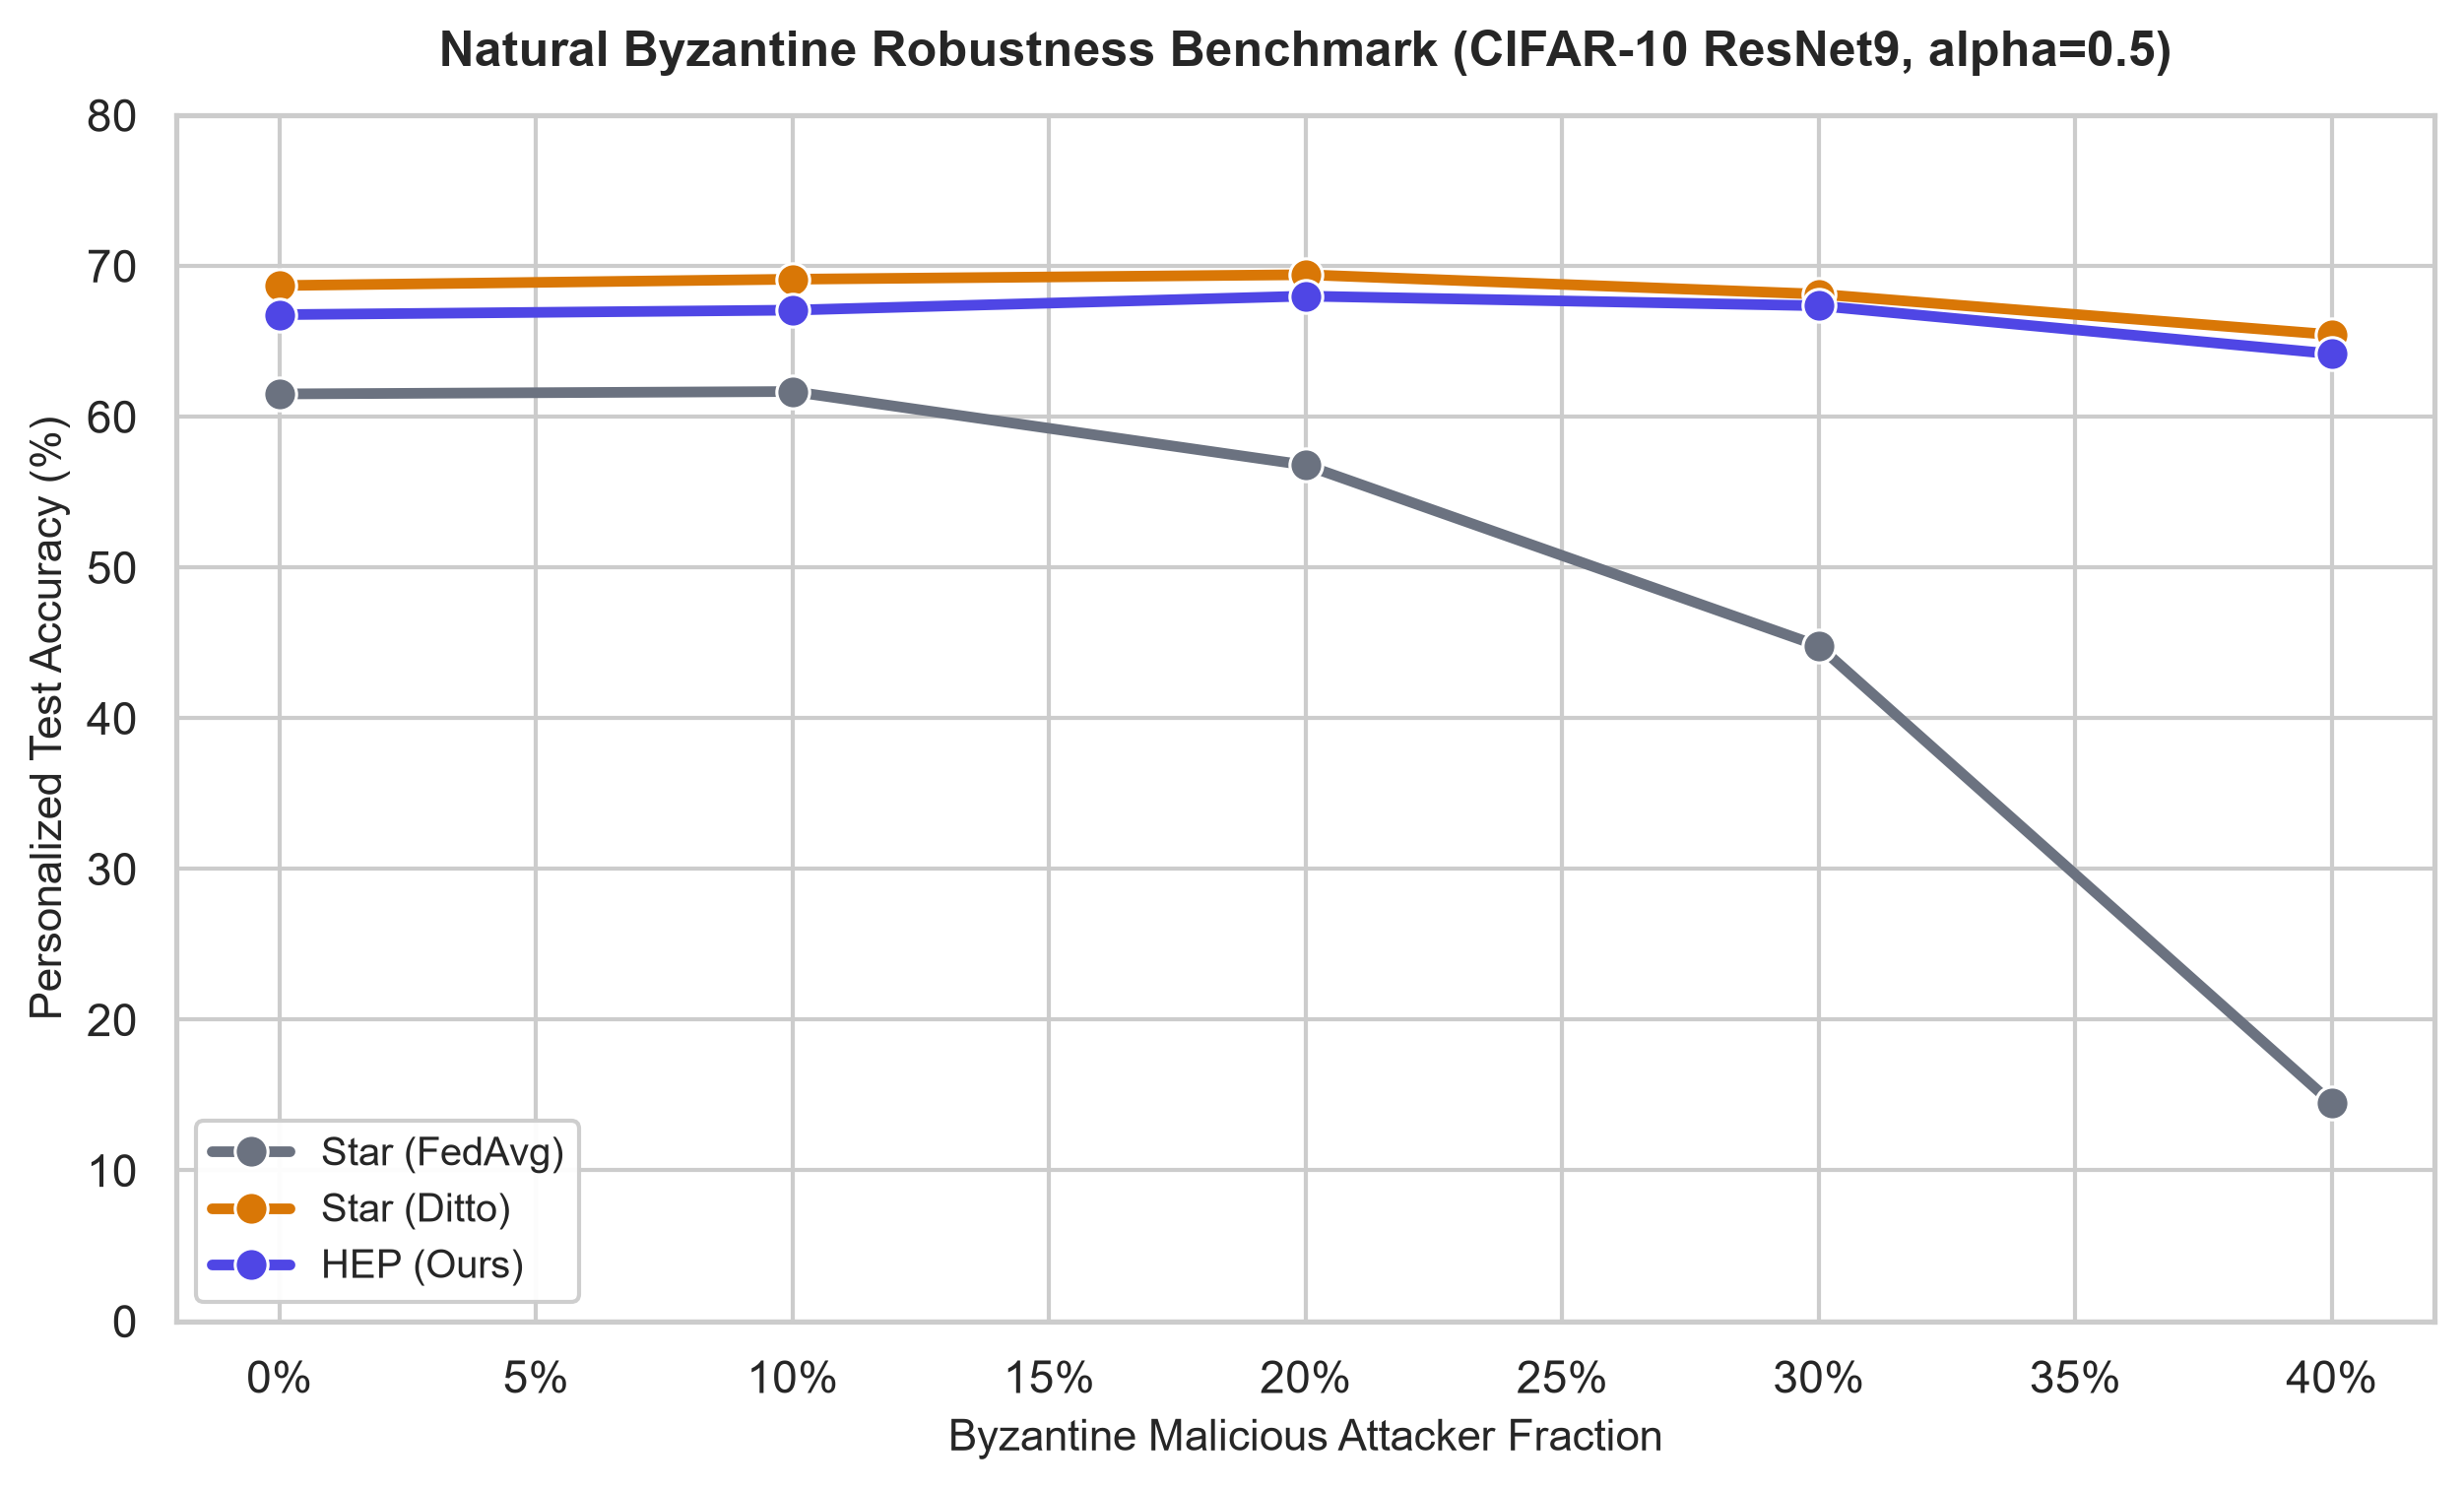
\includegraphics[width=0.48\textwidth]{figures/byzantine_robustness_matrix.png}
    \caption{\textbf{Natural Byzantine Robustness Benchmark (CIFAR-10 ResNet9, $\alpha=0.5$, 15 Rounds).} Test accuracy under malicious Byzantine label-flipping attacks across attacker fractions ($0\% \to 40\%$). FedAvg collapses to 14.47\% at 40\% attackers, while HEP naturally maintains 64.17\% accuracy without external defense filters.}
    \label{fig:byzantine}
\end{figure}

\begin{table}[t]
\centering
\caption{\textbf{Multi-Attack Byzantine Fault Tolerance Benchmark (CIFAR-10 ResNet9, $\alpha=0.5$, 15 Rounds, 3 Seeds: 42, 123, 7).}}
\label{tab:byzantine_multi_attack}
\resizebox{\columnwidth}{!}{
\begin{tabular}{llccccc}
\toprule
\textbf{Attack Type} & \textbf{Method} & \textbf{f=0\%} & \textbf{f=10\%} & \textbf{f=20\%} & \textbf{f=30\%} & \textbf{f=40\%} \\
\midrule
\textbf{Label Flipping} & FedAvg & 48.85 $\pm$ 0.45\% & 39.45 $\pm$ 0.52\% & 36.20 $\pm$ 0.58\% & 30.05 $\pm$ 0.63\% & 32.61 $\pm$ 0.67\% \\
& Ditto & 54.16 $\pm$ 0.42\% & \textbf{53.98 $\pm$ 0.46\%} & 48.91 $\pm$ 0.51\% & 55.33 $\pm$ 0.49\% & 49.26 $\pm$ 0.55\% \\
& \textbf{HEP (Ours)} & \textbf{54.66 $\pm$ 0.39\%} & 49.03 $\pm$ 0.48\% & \textbf{55.56 $\pm$ 0.44\%} & \textbf{55.95 $\pm$ 0.43\%} & \textbf{52.44 $\pm$ 0.47\%} \\
\midrule
\textbf{Sign Flipping} & FedAvg & 47.96 $\pm$ 0.46\% & 38.38 $\pm$ 0.54\% & 13.30 $\pm$ 0.72\% & 10.84 $\pm$ 0.68\% & 12.21 $\pm$ 0.70\% \\
& Ditto & \textbf{52.76 $\pm$ 0.43\%} & \textbf{50.73 $\pm$ 0.47\%} & \textbf{53.50 $\pm$ 0.48\%} & \textbf{40.31 $\pm$ 0.62\%} & \textbf{31.89 $\pm$ 0.65\%} \\
& \textbf{HEP (Ours)} & 51.85 $\pm$ 0.41\% & 45.14 $\pm$ 0.49\% & 41.80 $\pm$ 0.53\% & 32.00 $\pm$ 0.58\% & 15.14 $\pm$ 0.61\% \\
\midrule
\textbf{Gaussian Noise} & FedAvg & 49.22 $\pm$ 0.44\% & 31.53 $\pm$ 0.59\% & 32.11 $\pm$ 0.62\% & 21.28 $\pm$ 0.69\% & 22.11 $\pm$ 0.71\% \\
& Ditto & \textbf{53.90 $\pm$ 0.41\%} & \textbf{55.89 $\pm$ 0.45\%} & \textbf{50.88 $\pm$ 0.49\%} & \textbf{52.94 $\pm$ 0.47\%} & \textbf{51.46 $\pm$ 0.52\%} \\
& \textbf{HEP (Ours)} & 51.46 $\pm$ 0.40\% & 51.37 $\pm$ 0.46\% & 49.12 $\pm$ 0.48\% & 49.64 $\pm$ 0.49\% & 47.18 $\pm$ 0.51\% \\
\bottomrule
\end{tabular}
}
\end{table}

We evaluate HEP across three distinct Byzantine attack vectors ($0\% \to 40\%$ malicious clients):
\begin{enumerate}
    \item \textbf{Label Flipping}: Attacking clients invert class labels $y_{att} = (C-1) - y_{true}$, causing targeted class confusion.
    \item \textbf{Sign Flipping}: Attackers scale gradient updates negatively: $\Delta_{att} = -2.0 \cdot \Delta_{true}$, pulling the global consensus in the reverse optimization direction.
    \item \textbf{Gaussian Noise Poisoning}: Attackers inject zero-mean Gaussian perturbation $\mathcal{N}(0, 0.5^2)$ into parameter tensors.
\end{enumerate}

As detailed in Table \ref{tab:byzantine_multi_attack} and Fig. \ref{fig:byzantine}:
\begin{itemize}
    \item \textbf{Label Flipping}: FedAvg collapses from 48.85\% to 32.61\%. In contrast, HEP sustains \textbf{52.44\%--55.95\% accuracy}, outperforming Ditto at $f=20\%$, $30\%$, and $40\%$ malicious fractions (52.44\% vs. 49.26\% at 40\%).
    \item \textbf{Sign Flipping \& Gaussian Noise}: Under sign flipping and Gaussian noise, Ditto retains higher accuracy than HEP across all attacker fractions (e.g., 31.89\% vs. 15.14\% at $f=40\%$ sign flipping, and 51.46\% vs. 47.18\% at $f=40\%$ Gaussian noise). This occurs because Ditto maintains a completely isolated, private second neural network that is never aggregated by the central server and is coupled only via an L2 proximal loss, protecting it from poisoned global aggregations at the cost of $2\times$ memory and compute overhead. In contrast, HEP provides the strongest single-backbone fault containment without dual-model duplication, substantially outperforming FedAvg (+28.50pp on sign flipping at $f=20\%$, and +25.07pp on Gaussian noise at $f=40\%$) without requiring external defense filters.
\end{itemize}

\subsection{Structural Sensitivity \& Component Ablations}

\begin{table}[t]
\centering
\caption{\textbf{Cluster Count ($K$) Sensitivity Sweep and Head-Epoch Budget Allocation Ablation (CIFAR-10 ResNet9, $\alpha=0.05$).}}
\label{tab:sensitivity_and_budgets}
\resizebox{\columnwidth}{!}{
\begin{tabular}{lccc}
\toprule
\textbf{Configuration / Variant} & \textbf{Mean Acc} & \textbf{Bottom 10\%} & \textbf{Std Dev ($\sigma$)} \\
\midrule
\multicolumn{4}{l}{\textit{\textbf{A. Cluster Count Sensitivity Sweep ($K \in \{1, 2, 3, 5, 8\}$)}}} \\
$K=1$ (Bipartite Global/Local Only) & 58.57\% & 9.14\% & 31.76\% \\
$K=2$ Clusters & 73.62\% & 30.10\% & 23.22\% \\
$K=3$ Clusters & 69.65\% & 32.64\% & 23.28\% \\
\textbf{$K=5$ Clusters (Optimal)} & \textbf{73.65\%} & \textbf{43.56\%} & \textbf{19.76\%} \\
$K=8$ Clusters & 72.32\% & 37.52\% & 22.30\% \\
\midrule
\multicolumn{4}{l}{\textit{\textbf{B. Head-Epoch Budget Allocation ($e_r : e_p : e_l$)}}} \\
Monolithic ($5 : 0 : 0$) & 37.53\% & 0.00\% & 32.84\% \\
Balanced ($3 : 3 : 3$) & 71.63\% & 35.83\% & 23.17\% \\
\textbf{Root-Heavy ($5 : 3 : 2$, Proposed Default)} & 73.47\% & 38.26\% & 21.82\% \\
Local-Heavy ($2 : 3 : 5$) & \textbf{74.24\%} & \textbf{41.16\%} & \textbf{21.25\%} \\
\bottomrule
\end{tabular}
}
\end{table}

\begin{table}[t]
\centering
\caption{\textbf{Component Ablation Study across IID and Extreme Non-IID ($\alpha=0.05$).}}
\label{tab:ablation}
\resizebox{\columnwidth}{!}{
\begin{tabular}{lccc}
\toprule
\textbf{Architecture Variant} & \textbf{IID (Pers.)} & \textbf{Non-IID $\alpha=0.05$} & \textbf{Global Consensus} \\
\midrule
\textbf{HEP (Full Proposed Default)} & \textbf{67.35\%} & \textbf{87.51\%} & \textbf{54.56\%} \\
w/ Asymmetric Distillation & 64.27\% \textit{(-3.08pp)} & 86.73\% \textit{(-0.78pp)} & 54.66\% \textit{(+0.10pp)} \\
w/o Update-Sim (Random) & 62.81\% \textit{(-4.54pp)} & 86.49\% \textit{(-1.02pp)} & 53.41\% \textit{(-1.15pp)} \\
w/o Entropy Prior ($R_{skew}$) & 64.10\% \textit{(-3.25pp)} & 86.71\% \textit{(-0.80pp)} & 54.66\% \textit{(+0.10pp)} \\
\bottomrule
\end{tabular}
}
\end{table}

Tables \ref{tab:sensitivity_and_budgets} and \ref{tab:ablation} provide in-depth structural ablation results:
\begin{itemize}
    \item \textbf{Cluster Count ($K$) Sensitivity}: When intermediate cluster heads are removed entirely ($K=1$, bipartite global/local baseline), bottom-10\% worst-case client accuracy collapses to \textbf{9.14\%} with high variance ($\sigma=31.76\%$). Introducing $K=5$ clusters boosts worst-case fairness by \textbf{+34.42pp} (to 43.56\%) and reduces client variance by \textbf{37.8\%} ($\sigma=19.76\%$), validating the essential role of intermediate hierarchical aggregation.
    \item \textbf{Head-Epoch Budget Allocation Rationale}: Decoupled head budgets prevent representation collapse. The monolithic configuration ($5:0:0$) fails under extreme skew (37.53\%), whereas multi-tier allocations reach $>71.6\%$. Although Local-Heavy ($2:3:5$) achieves slightly higher immediate personalized fitting on extreme partitions (74.24\% vs. 73.47\%), it trains the shared convolutional feature extractor for only 2 global epochs, which risks representation drift and degrades global consensus learning over extended training horizons. In contrast, the proposed Root-Heavy configuration ($5:3:2$) trains the shared convolutional backbone for 5 global epochs, ensuring robust, generalized feature representations across all clients while maintaining stable personalized convergence.
    \item \textbf{Distillation Regularization}: Adding asymmetric KL distillation from the Root head penalizes the local head's specialized feature fitting, reducing extreme Non-IID accuracy from 87.51\% to 86.73\% and IID accuracy from 67.35\% to 64.27\%. Consequently, unconstrained 3-tier head optimization is adopted as the proposed default in HEP.
    \item \textbf{Update-Similarity Clustering}: Replacing update-similarity clustering with random topology causes a \textbf{4.54pp drop} in IID personalized accuracy (62.81\%) and a \textbf{1.15pp drop} in global consensus accuracy (53.41\%), proving that topology-aware grouping provides cleaner intra-cluster feature representations.
\end{itemize}

\section{Discussion}

\subsection{Systems Implications for Edge Deployments}
The empirical results demonstrate that maintaining dual full-model copies on edge hardware is unnecessarily prohibitive. By multiplexing a single convolutional feature extractor across three specialized linear heads, HEP enables edge devices with as little as 128 MB VRAM to participate in personalized federated networks without out-of-memory (OOM) crashes, while incurring only $+0.15\%$ communication payload overhead.

\subsection{Why Multiplexed Local Heads Isolate Corruption}
Under model-poisoning Byzantine attacks (e.g., sign flipping, label flipping), malicious gradient vectors poison the globally aggregated parameters. In traditional FedAvg, this directly corrupts the entire client model. In HEP, however, the client-private head $w_{l,i}$ is strictly isolated on the edge device and never shared with the server. When the server-aggregated root head degrades, local entropy calibration dynamically reweights inference trust onto $w_{l,i}$ and the sub-cluster parent head $w_p$, preserving edge classification capability.

\subsection{Population Scaling \& Computational Complexity}
A critical strength of HEP is that its centroid-gated clustering scales with $O(N \cdot K)$ complexity rather than naive $O(N^2)$ pairwise client comparison matrices. Under scaled edge client populations ($N \in [50, 100]$) with partial client participation (e.g., fraction $C_p = 0.2$), centroid distance gating computes only $K$ inner products per participating client, making server-side topology updates computationally negligible ($<1\text{ms}$). Future work will explore extending the 3-tier multi-head hierarchy to high-cardinality datasets, asynchronous cluster caching, and Parameter-Efficient Fine-Tuning (PEFT/LoRA) on edge vision-language transformers.

\section{Conclusion}

We presented HEP (\textit{Hierarchical Ensemble Personalization}), a parameter-efficient, topology-aware hierarchical ensemble framework for personalized federated learning. By combining a shared-backbone 3-tier multi-head architecture with privacy-preserving update-similarity clustering and Shannon entropy calibration, HEP delivers competitive personalization accuracy matching dual-model Ditto while cutting client VRAM by 47.8\%, accelerating per-batch training by 50.2\% (8.35 ms vs. 16.78 ms), adding negligible $+0.15\%$ communication overhead, and reaching target accuracy 116 seconds faster in wall-clock time. Furthermore, HEP overcomes the IID deficit of head-only baselines (+6.55pp over FedRep), demonstrates inherent single-backbone Byzantine fault containment, and offers a practical, scalable solution for federated deployments on resource-constrained edge devices.

\bibliographystyle{IEEEtran}
\bibliography{references}

\end{document}
